Przyjrzymy się więc jednej stronie powyższego dualizmu i przeanalizujmy kopuły jako struktury zależności.

\begin{df}[Kopuła minimum]
	Dwuwymiarowa kopuła minimum $C^{-}$ to kopuła zadana wzorem $C^{-}(u, v) = \max(u+v-1, 0).$
\end{df}
\begin{df}[Kopuła maximum]
	Dwuwymiarowa kopuła maksimum $C^{+}$, to kopuła zadana wzorem $C^{+}(u, v) = \min(u, v).$
\end{df}

\begin{figure}[h]
	\centering
	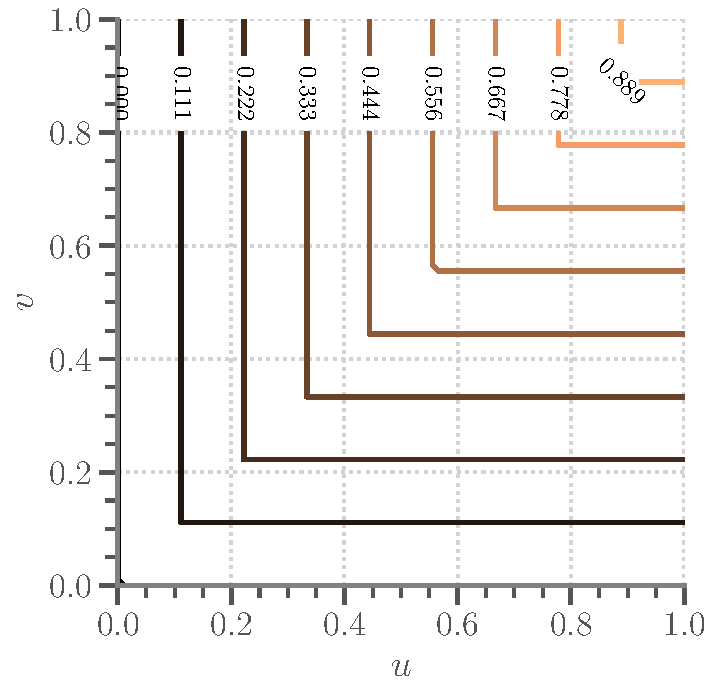
\includegraphics[width=0.35\linewidth]{02_MaximumCopula_contour}
	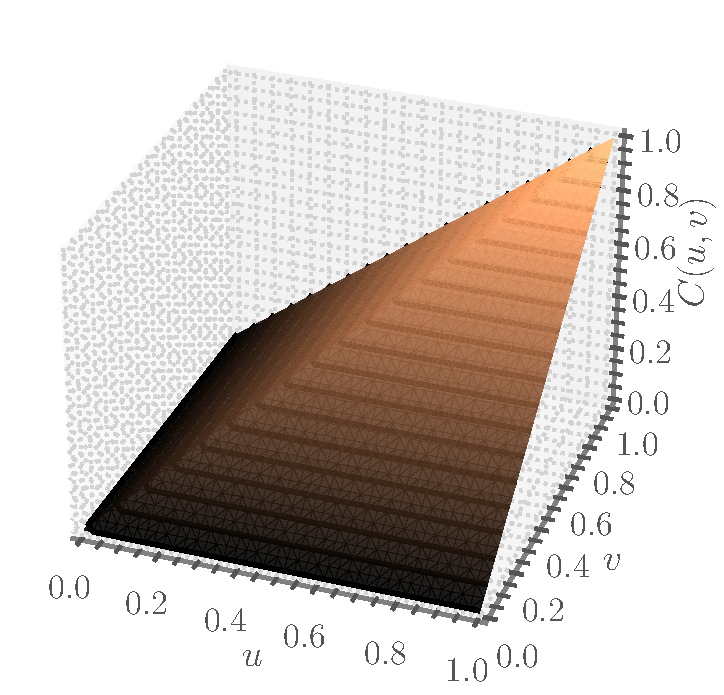
\includegraphics[width=0.4\linewidth]{02_MaximumCopula_surface}
	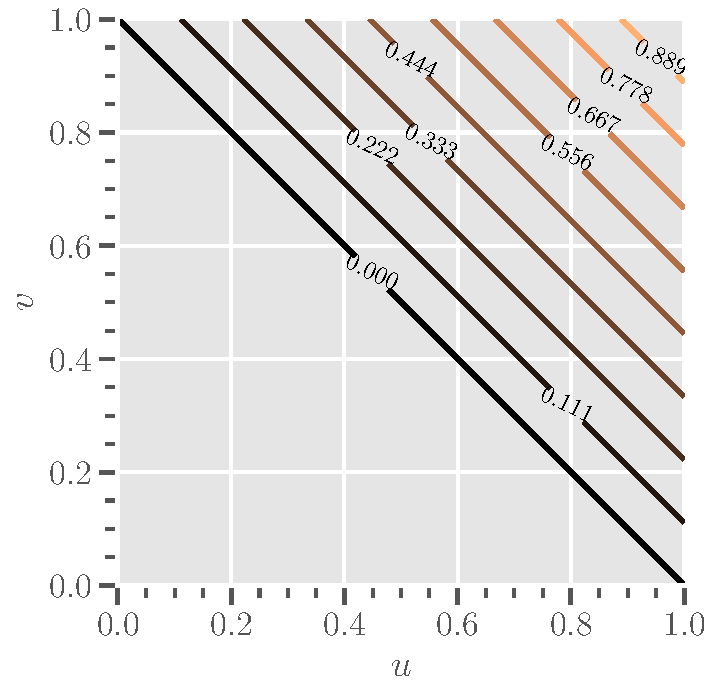
\includegraphics[width=0.35\linewidth]{02_MinimumCopula_contour}
	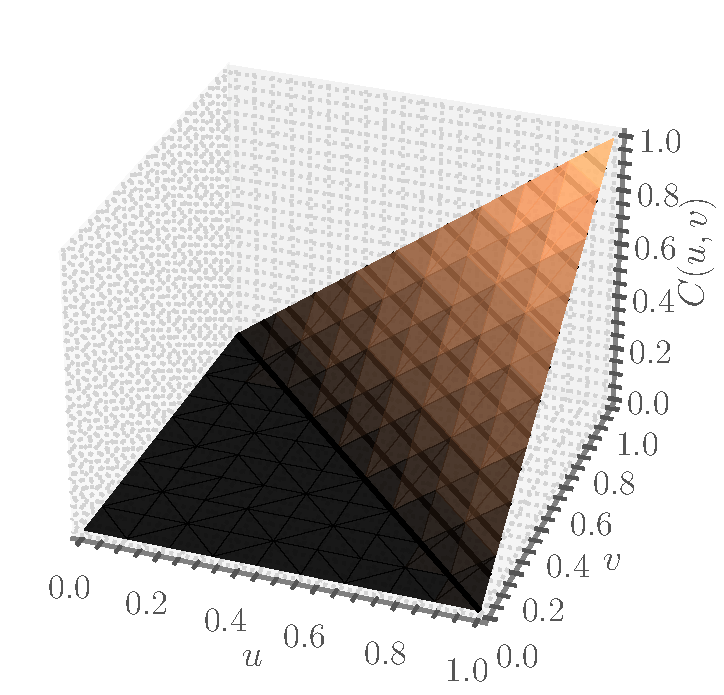
\includegraphics[width=0.4\linewidth]{02_MinimumCopula_surface}
	
	\caption{\textbf{Kopuły minimum i maksimum.} Kontury (po lewej) i dystrybuanty (po prawej) kopuł: maximum (górny panel) i minimum (dolny panel)\label{fig:minmax_copula}}
\end{figure}

Kopuły minimum i maximum stanowią horyzont osiągalnych kopuł, ponieważ jak mówi twierdzenie \ref{thm:frechet_hoeffding}, są one ograniczeniem dolnym i górnym dla dowolnej innej kopuli. Ich powierzchnie i kontury przedstawia rysunek \ref{fig:minmax_copula}. 

\begin{thm}[Fréchet-Hoeffding bounds]
	Niech $C$ będzie $2$-wymiarową kopułą. Wtedy dla każdego $(u, v)\in[0, 1]^2$ zachodzi
	
	$$ C^{-}(u, v) \leqslant C(u, v) \leqslant C^{+}(u, v).$$
	
	\label{thm:frechet_hoeffding}
\end{thm}

Twierdzenie to, choć z pozoru teoretyczne, ciągnie za sobą bardzo praktyczne konsekwencje: pozwala otrzymać niezależne od modelu ogranicznia górne i dolne na dowolną kopułę. \cite{Cherubini_Copula_Methods_in_Finance} pokazuje przykład, w którym twierdzenie \newline Frécheta-Hoeffdinga pozwala na uzyskanie dolnego i górnego ograniczenia na pewne statystyki modelu, jak np. łączne prawdopodobieństwo bankructwa dwóch firm w strukturalnym modelu Mertona, czy cena opcji binarnej na dwa aktywa.\\

\begin{df}[Kopuła produktowa]
	Dwuwymiarowa kopuła produktowa $C^{\perp}$ to kopuła zadana wzorem $C^{\perp}(u, v) = uv.$
\end{df}

\begin{figure}[h]
	\centering
	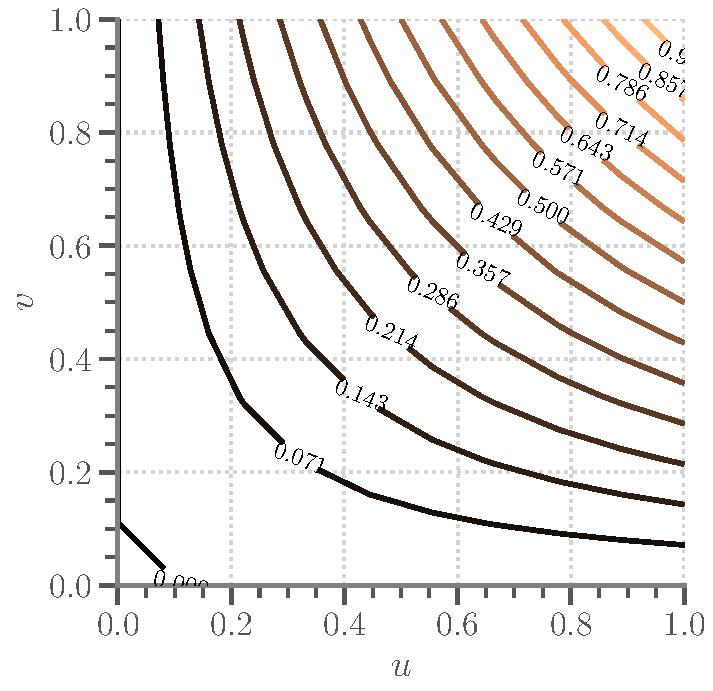
\includegraphics[width=0.35\linewidth]{02_ProductCopula_contour}
	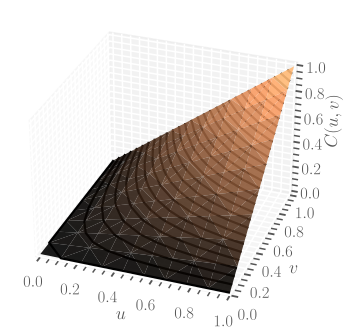
\includegraphics[width=0.4\linewidth]{02_ProductCopula_surface}
	
	\caption{\textbf{Kopuła produktowa.} Kontur (po lewej) i dystrybuanta (po prawej). \label{fig:prod_copula}}
\end{figure}

Kopuła produktowa jest trzecim istotnym punktem odniesienia w świecie kopuł, ponieważ posiada pewną unikalną właśność. Z jednej strony z definicji kopuły mamy:

\begin{equation}
C(u, v) = \Pra(U \leqslant u, V \leqslant v )
\label{eq:independence_copula1}
\end{equation}

Z drugiej jednak strony, wiemy że $U$ i $V$ mają rozkłady jednostajne - więc:
\begin{equation}
	F_U(u) = \Pra(U \leqslant u) = u\text{, oraz } F_V(v) = \Pra(V \leqslant v) = v.
\label{eq:independence_copula2}
\end{equation}

Z równań \ref{eq:independence_copula1} i \ref{eq:independence_copula2}, dla przypadku kopuły produktowej mamy zatem:
\begin{equation}
	\Pra(U \leqslant u, V \leqslant v ) \equiv C^{\perp}(u, v) = uv = \Pra(U \leqslant u) \Pra(V \leqslant v).
	\label{eq:independence_copula}
\end{equation}

Równanie \ref{eq:independence_copula} mówi nam, że zmienne losowe $V$ i $U$ są od siebie niezależne. Model kopuły produktowej, implikuje więc niezależność jednostajnych rozkładów brzegowych.\\
Co więcej, uzupełniając opis kopuł minimum i maksimum - te z kolei odpowiadają współmonotonicznej i przeciwmonotonicznej zależności jednostajnych rozkładów brzegowych. Rodzinę kopuł zawierającą w sobie $C^{-}, C^{\perp}$, oraz $C^{+}$ nazywać będziemy kompletną \emph{(eng. comprehensive)}. Widzimy zatem, że kopuły potrafią modelować pełne spektrum możliwych zależności: od współmonotonicznych, przez niezależne, aż po przeciwmonotoniczne.\\

\begin{prop}[$\rho$ Spearmana i $\tau$ Kendalla]
	Dla $X$ i $Y$: ciągłych zmiennych losowych o kopule $C$ możemy przedstawić $\tau$ Kendalla jako:
	
	\begin{equation}
		\tau = 4\int\int_{[0, 1]^2}C(u,v)dC(u,v) -1.
		\label{eq:tau_from_copula}
	\end{equation}
	Współczynnik korelacji Spearmana $\rho$ można przedstawić natomiast w postaci:
	\begin{equation}	
		\rho = 12\int\int_{[0, 1]^2}uvdC(u,v) -3.
		\label{eq:rho_from_copula}
	\end{equation}
	\label{thm:tau_from_copula}
\end{prop}

Przypomnijmy, że w rozdziale \ref{sec:miary_współzależności} połączyliśmy wspoł- i przeciwmonotoniczność z miarami zgodności. Istotnie, bezpośrednio ze wzorów \ref{eq:tau_from_copula} i \ref{eq:rho_from_copula} otrzymujemy teraz dla $C^{+}$: $\tau=1$ oraz $\rho=1$, dla $C^{\perp}$: $\tau=0$ i $\rho=0$, natomiast dla $C^{-}$ mamy $\tau=-1$ i $\rho=-1$. Wzory z własności \ref{thm:tau_from_copula} mają jednak głębsze znaczenie: zadają bijekcję (niezależną od rozkładów brzegowych) między miarami zgodności a konkretną kopułą. Z tego powodu, estymacja $\tau$ jest równoważna estymacji parametrów kopuły, co jest wykorzystywane do kalibracji.

Podobnie jest ze wspołczynnikami zależności ogonów, wprowadzonymi w rozdziale \ref{sec:miary_współzależności}. Wprost z definicji kopuły wynika, że można je przedstawić używając jedynie kopuły:
\begin{prop}[Zależność ogonów]
		Górny współczynnik zależności ogonów $(X_1, X_2)$ o rozkładach brzegowych $F_1$ i $F_2$ i kopuli $C$ możemy przedstawić jako:
		$$ \lambda^{u} = \lim\limits_{t\to1^{-}}\Pra[X_2 > F_2^{-1}(t) \vert X_1 > F_1^{-1}(t) ] = \lim\limits_{t\to1^{-}}\frac{1-2t+C(t, t)}{1-t}.$$
		Dolny współczynnik możemy przedstawić natomiast w postaci:
		$$ \lambda^{l} = \lim\limits_{t\to0^{+}}\Pra[X_2 \leqslant F_2^{-1}(t) \vert X_1 \leqslant F_1^{-1}(t) ] = \lim\limits_{t\to0^{+}}\frac{C(t, t)}{t}.$$
\end{prop}